% Use xelatex to generate a pdf file of this presentation

\documentclass{beamer}
\usepackage{roboto}
\usepackage[russian]{babel}
\usetheme{Copenhagen}

% Simple way to put a code listing to the slide
\usepackage{listings}

\usepackage{tikz}
\usepackage{graphicx}
  \logo{
\includegraphics[scale=0.05]{pics/elephant}}

\addtobeamertemplate{frametitle}{}{
\begin{tikzpicture}[remember picture,overlay]
\node[anchor=north east] at (current page.north east) {
\includegraphics[height=0.6cm]{pics/garuda.png}};
\end{tikzpicture}
}

% Blocks settings
\setbeamerfont{block title}{size=\tiny}
%\setbeamersize{text margin left = -5pt, text margin right = -5pt}

% https://pgday.org.il
%Information to be included in the title page:
\title{Does PostgreSQL respond}
\subtitle{to the challenge of analytical queries?}
\author{Lepikhov Andrey}
\institute{PostgreSQL Thailand Development Group}
\date{2024}

% Add page numbers in the footnote
\expandafter\def\expandafter\insertshorttitle\expandafter{%
  \insertshorttitle\hfill%
  \insertframenumber\,/\,\inserttotalframenumber}

\definecolor{lightlightgray}{gray}{0.9}

% Default listing format
\lstset{language=sql, frame=none, tabsize=2, identifierstyle=\color{black},
  showspaces=false, showtabs=false, showstringspaces=false,
  columns=fullflexible, % Restore default spaces between letters
  basicstyle=\rmfamily\scriptsize,
  stringstyle=\color{purple},
  keywordstyle=\bfseries\color{green!40!black},
  numberstyle=\tiny\color{gray}}

% -----------------------------

\begin{document}

% %%%%%%%%%%%%%%%%%%%%%%%%%%%%%%%%%%%%%%%%%%%%%%%%%%%%%%%%%%%%%%%%%%%%%%%%
% General idea: having lots of reports on issues during migrations, I discovered the code and its dynamics to understand whether we have a chance to help users resolve their problems or this state for a long time
% %%%%%%%%%%%%%%%%%%%%%%%%%%%%%%%%%%%%%%%%%%%%%%%%%%%%%%%%%%%%%%%%%%%%%%%%

\begin{frame}
\titlepage
   \tikz [remember picture,overlay]
    \node at
        ([yshift=2.0cm, xshift=-4.5cm]current page.center) 
        {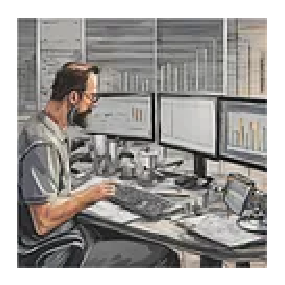
\includegraphics[scale=0.3]{pics/project_logo}};
   \tikz [remember picture,overlay]
    \node at
        ([yshift=2.0cm, xshift=+4.5cm]current page.center) 
        {
\includegraphics[scale=0.18]{pics/garuda.png}};
   \tikz [remember picture,overlay]
    \node at
        ([yshift=-2.5cm, xshift=0cm]current page.center) 
        {\includegraphics[scale=0.025]{pics/flag_of_Thailand.png}};
\end{frame}
% I would like to talk now about analytics and Postgres.
% The reason is the diverse usage of this database system initially designed for transactional load.
% For good or bad, I observe a wave of Oracle and SQL Server migrations to PostgreSQL.
% And many reports are raised about performance degradation of specific queries.
% Analysing these cases, I see that some technological advancements of these DBMSes usually cause them.
% Almost all cases are caused by queries that users name 'analytical queries'.
% So I've done this work to understand how safe it is to use Postgres and whether we can improve the situation soon.
% Or our clients should rewrite their queries and/or schema to tackle their problems.

\begin{frame}[fragile]\frametitle{Self Introduction}
\begin{itemize}
  \item 2007 - First touch to PostgreSQL (distributed query execution)
  \item 2010 - designer and user of databases based on PostgreSQL (and SQLite)
  \item 2017 - now - PostgreSQL Enthusiast, sporadic contributor and patch reviewer
\end{itemize}
My projects:
\begin{itemize}
  \item Multimaster, Shardman, Joinsel
  \item AQO, sr\_plan, SwitchJoin, re-optimisation ...
  \item Patches: GROUP-BY, Self-Join Removal, OR->ANY Optimisation ...
\end{itemize}
\end{frame}

\begin{frame}\frametitle{Purpose}
\begin{itemize}
  \item The scope of the analytic queries problem
  \item What is the PostgreSQL current progress?
  \item What is needed to be done (compared to over DBMSes)?
\end{itemize}
\end{frame}

\begin{frame}\frametitle{The risky tendency}
\begin{columns}\begin{column}{0.4\textwidth}
\begin{itemize}
  \item YugaByte
  \item Shardman
  \item Crunchy Data DuckDB integration
\end{itemize}
\end{column}
\begin{column}{0.6\textwidth}
  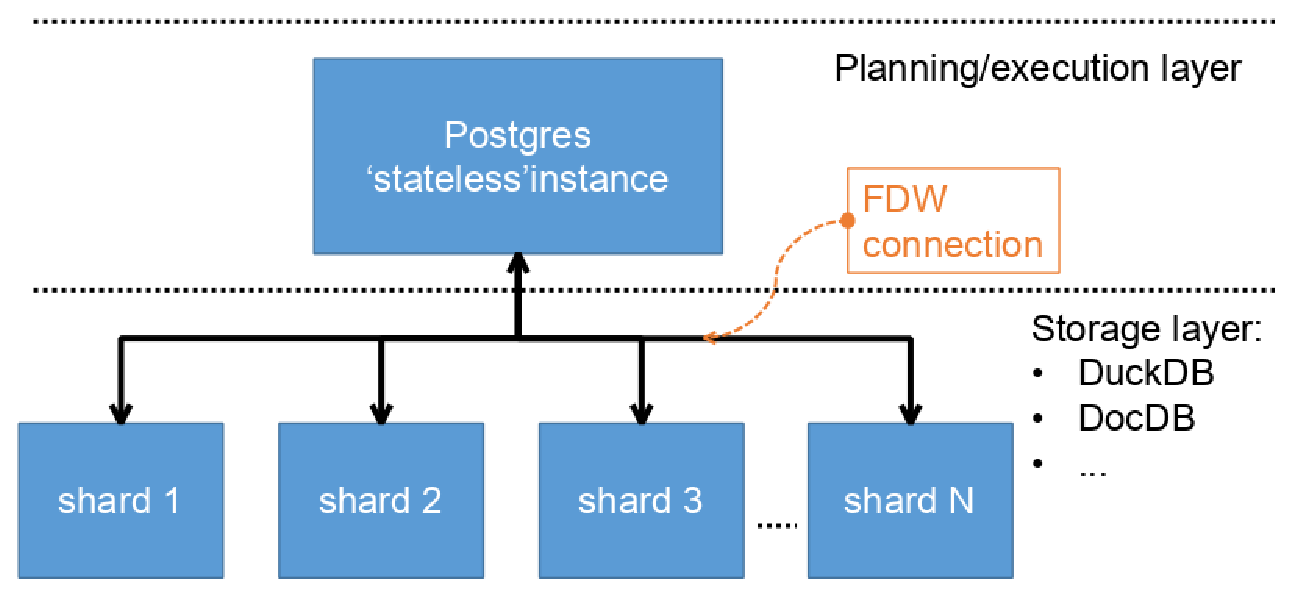
\includegraphics[scale=0.3]{pics/split_dbms}
\end{column}\end{columns}
%\vspace{5mm}
\bigskip
Greenplum, Citus, and Postgres-XL altered the Postgres optimiser code. However, the new approach uses Postgres almost 'as is'.
\end{frame}
% They assume that using highly effective storage for big data, they could manage it using the well-known Postgres DBMS as an interface.
% But the question is whether Postgres is ready to create effective query plans for partitioned data.

\begin{frame}\frametitle{What is analytic query?}
\begin{itemize}
  \item It touches a massive part of the tuples in a relation
  \item Uses a mix of aggregate functions over the same data
  \item Have a complex query structure (join tree, groupings, limits, sortings, etc)
  \item Actively uses subqueries and CTEs
  \item Relations are burdened with many indexes
\end{itemize}
\end{frame}

\begin{frame}\frametitle{What is the real progress?}
\begin{columns}\begin{column}{0.6\textwidth}
	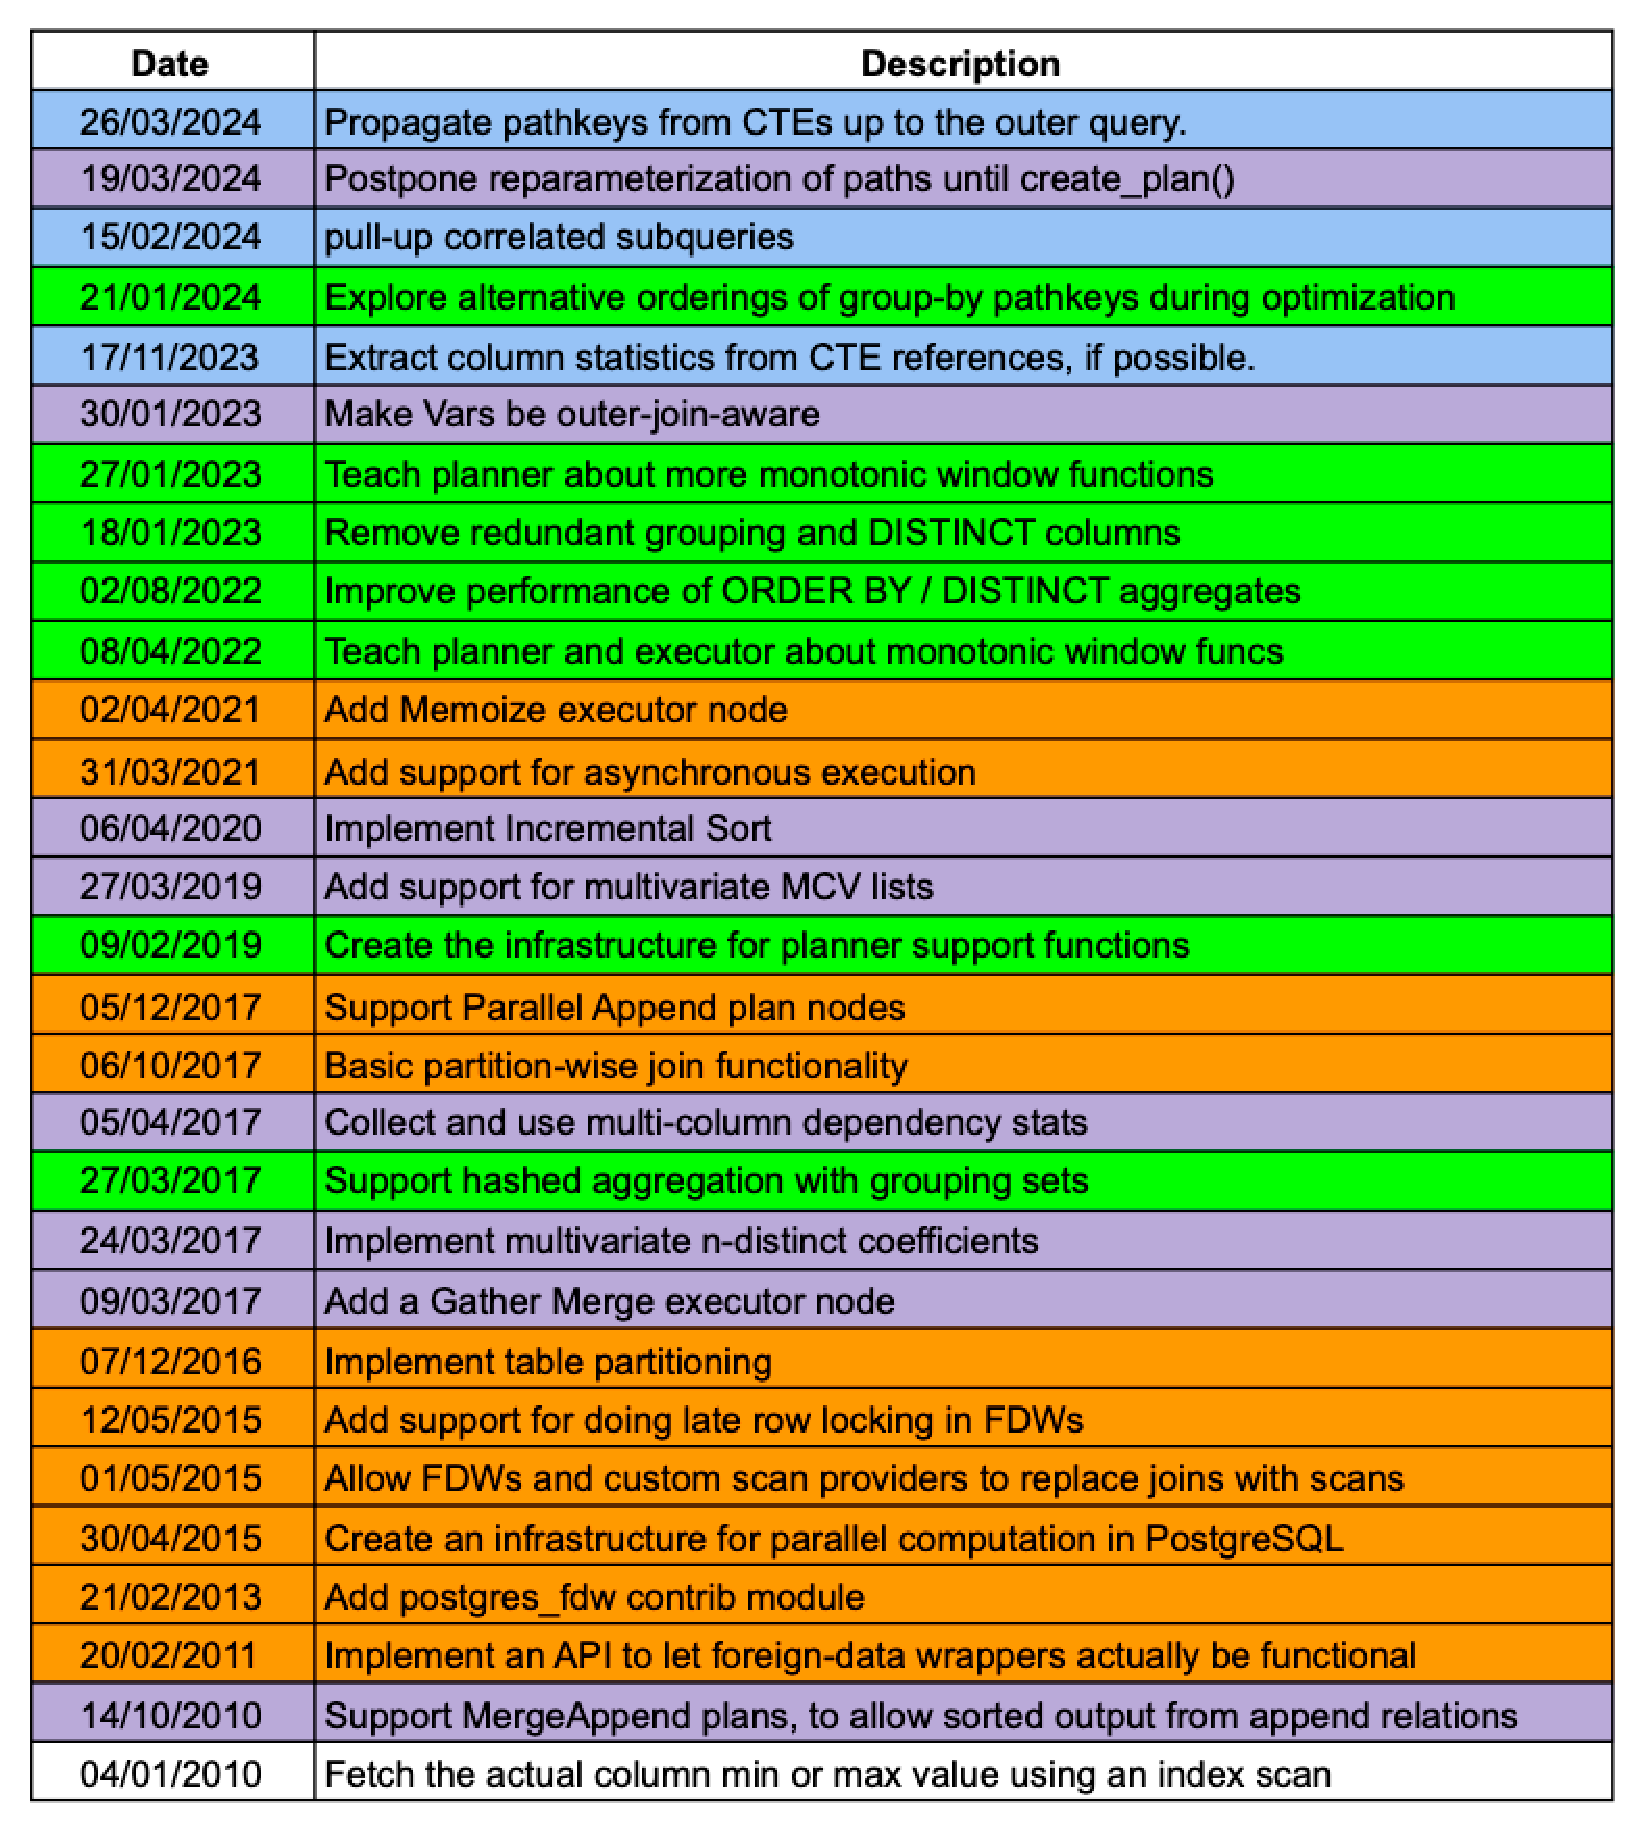
\includegraphics[scale=0.23]{pics/commits}
\end{column}
\begin{column}{0.5\textwidth}
\begin{itemize}
  \item \colorbox{orange}{Big storage}
  \item \colorbox{green}{Aggregates}
  \item \colorbox{purple!40}{Query structure}
  \item \colorbox{blue!40}{Subqueries \& CTEs}
  \item Indexes
\end{itemize}
\end{column}\end{columns}
\end{frame}

\begin{frame}\frametitle{Answer to fast-growing data storage}
\begin{itemize}
  \item Split data into partitions
  \item Distribute data (foreign data wrappers)
  \item Parallel execution techniques
  \item Smart caching (Memoize, Materialize)
\end{itemize}
\end{frame}

\begin{frame}
\vspace*{\fill}\begin{center}
Smart caching
\end{center}\vspace*{\fill}
\end{frame}

\begin{frame}\frametitle{Materialize}
	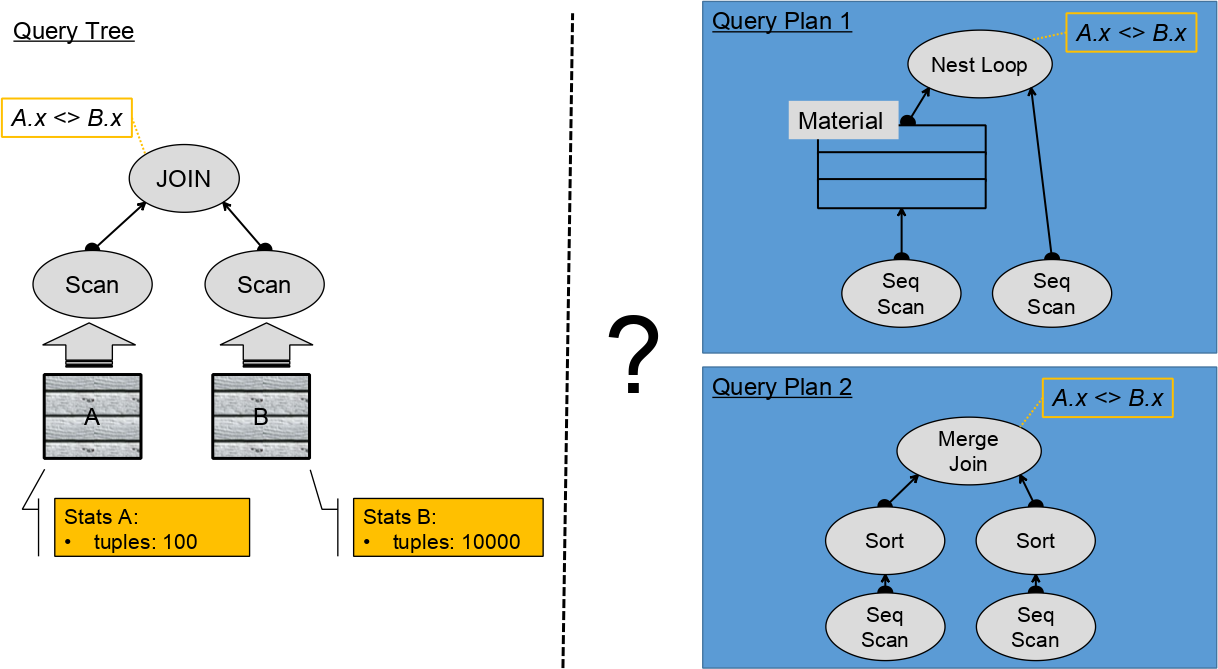
\includegraphics[scale=0.35]{pics/material}
\end{frame}

\begin{frame}[fragile]\frametitle{What's more with materialization?}
\begin{lstlisting}
SELECT * FROM a LEFT JOIN foreign_table_b b1
ON b1.x IN (
  SELECT y FROM foreign_table_b b2
  WHERE b1.z=a.z
);
\end{lstlisting}
\end{frame}

\begin{frame}\frametitle{What's more with materialization? - II}
	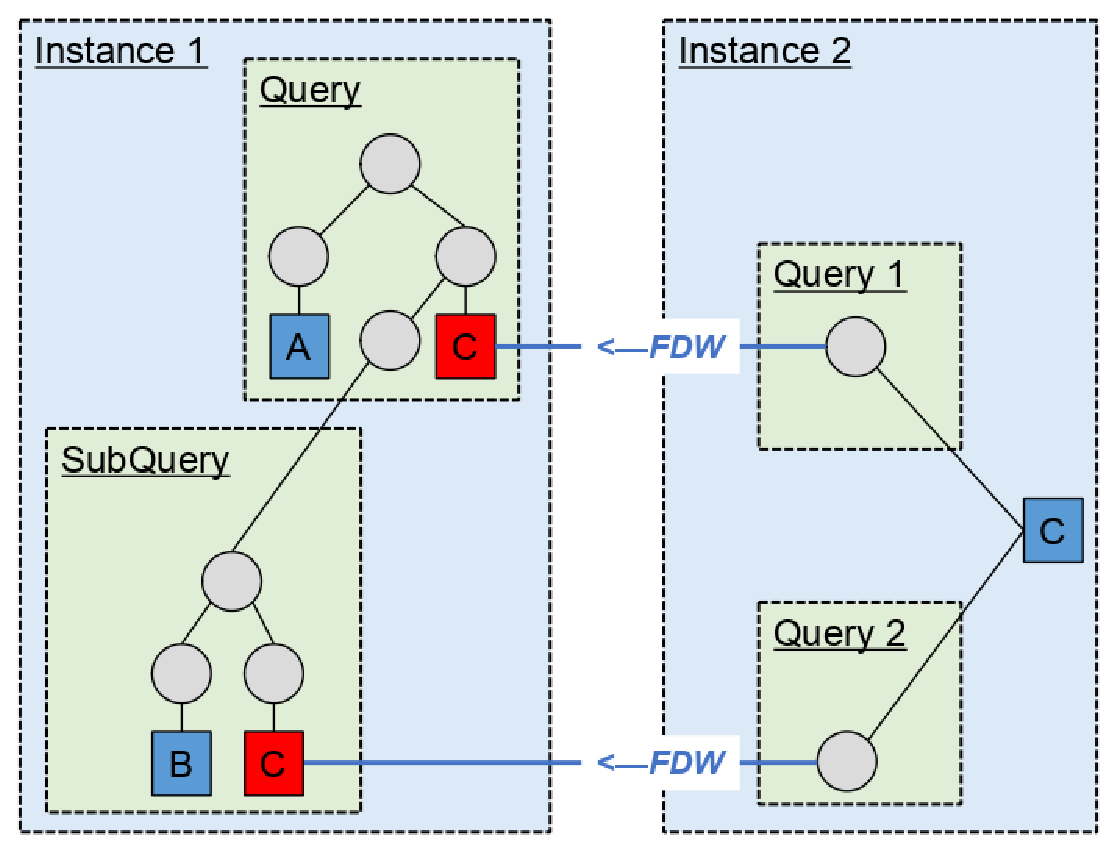
\includegraphics[scale=0.47]{pics/material_show_problem}
\end{frame}

\begin{frame}\frametitle{Cross-query materialization}
	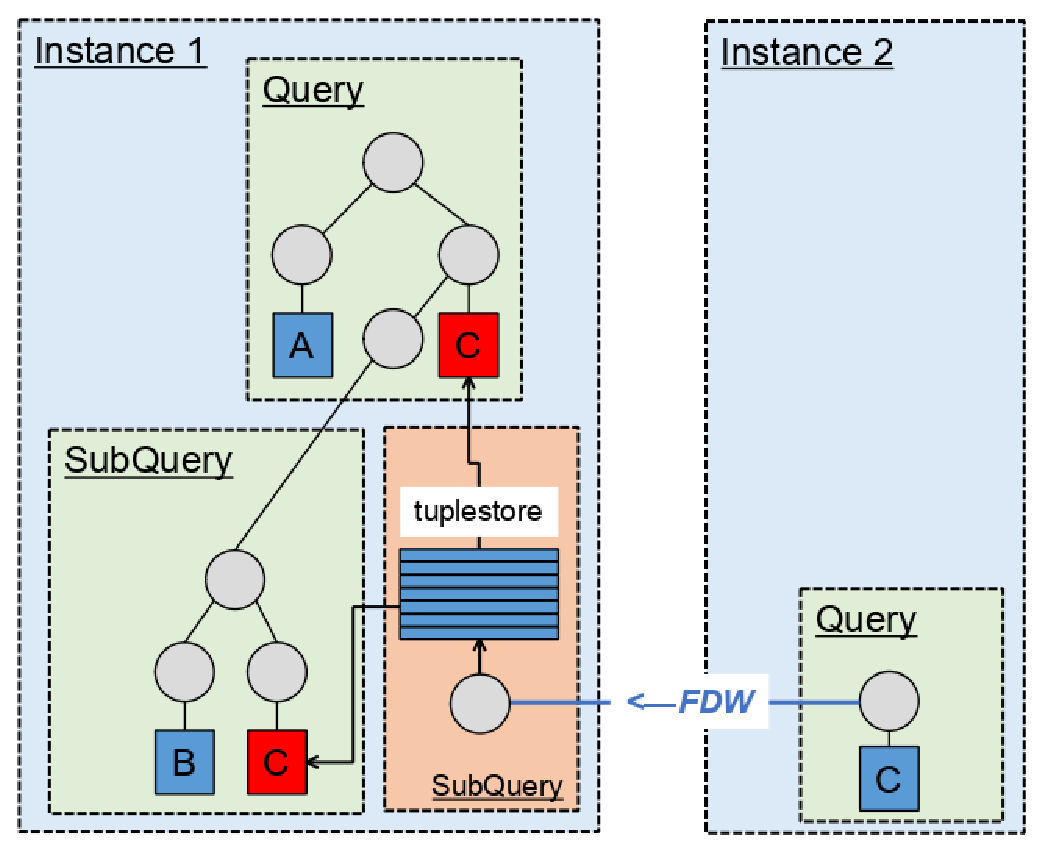
\includegraphics[scale=0.5]{pics/tee}
\end{frame}

\begin{frame}\frametitle{Memoize}
  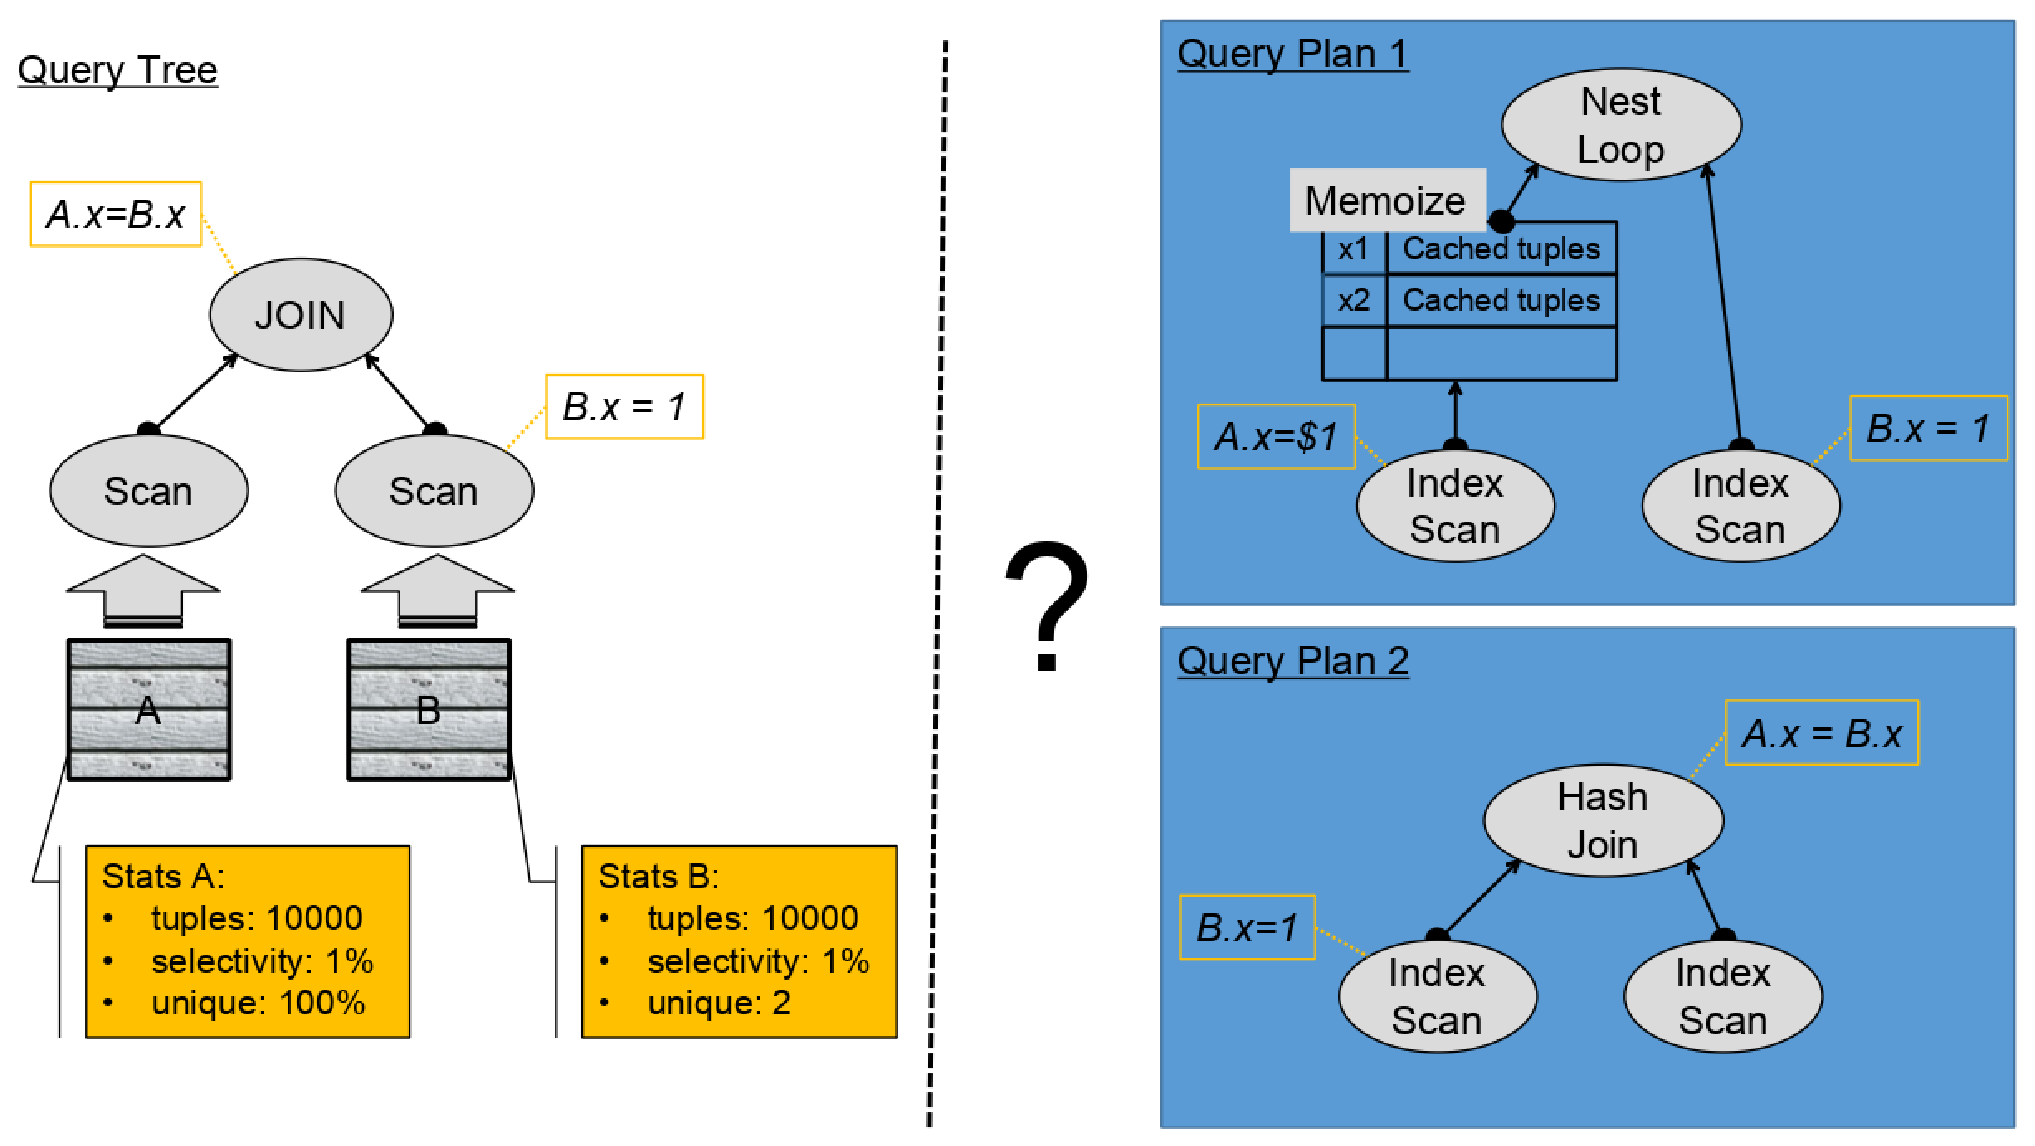
\includegraphics[scale=0.32]{pics/memoize}
\end{frame}

\begin{frame}\frametitle{Memoization: What's more?}
%\begin{center}
\hspace*{\fill}
	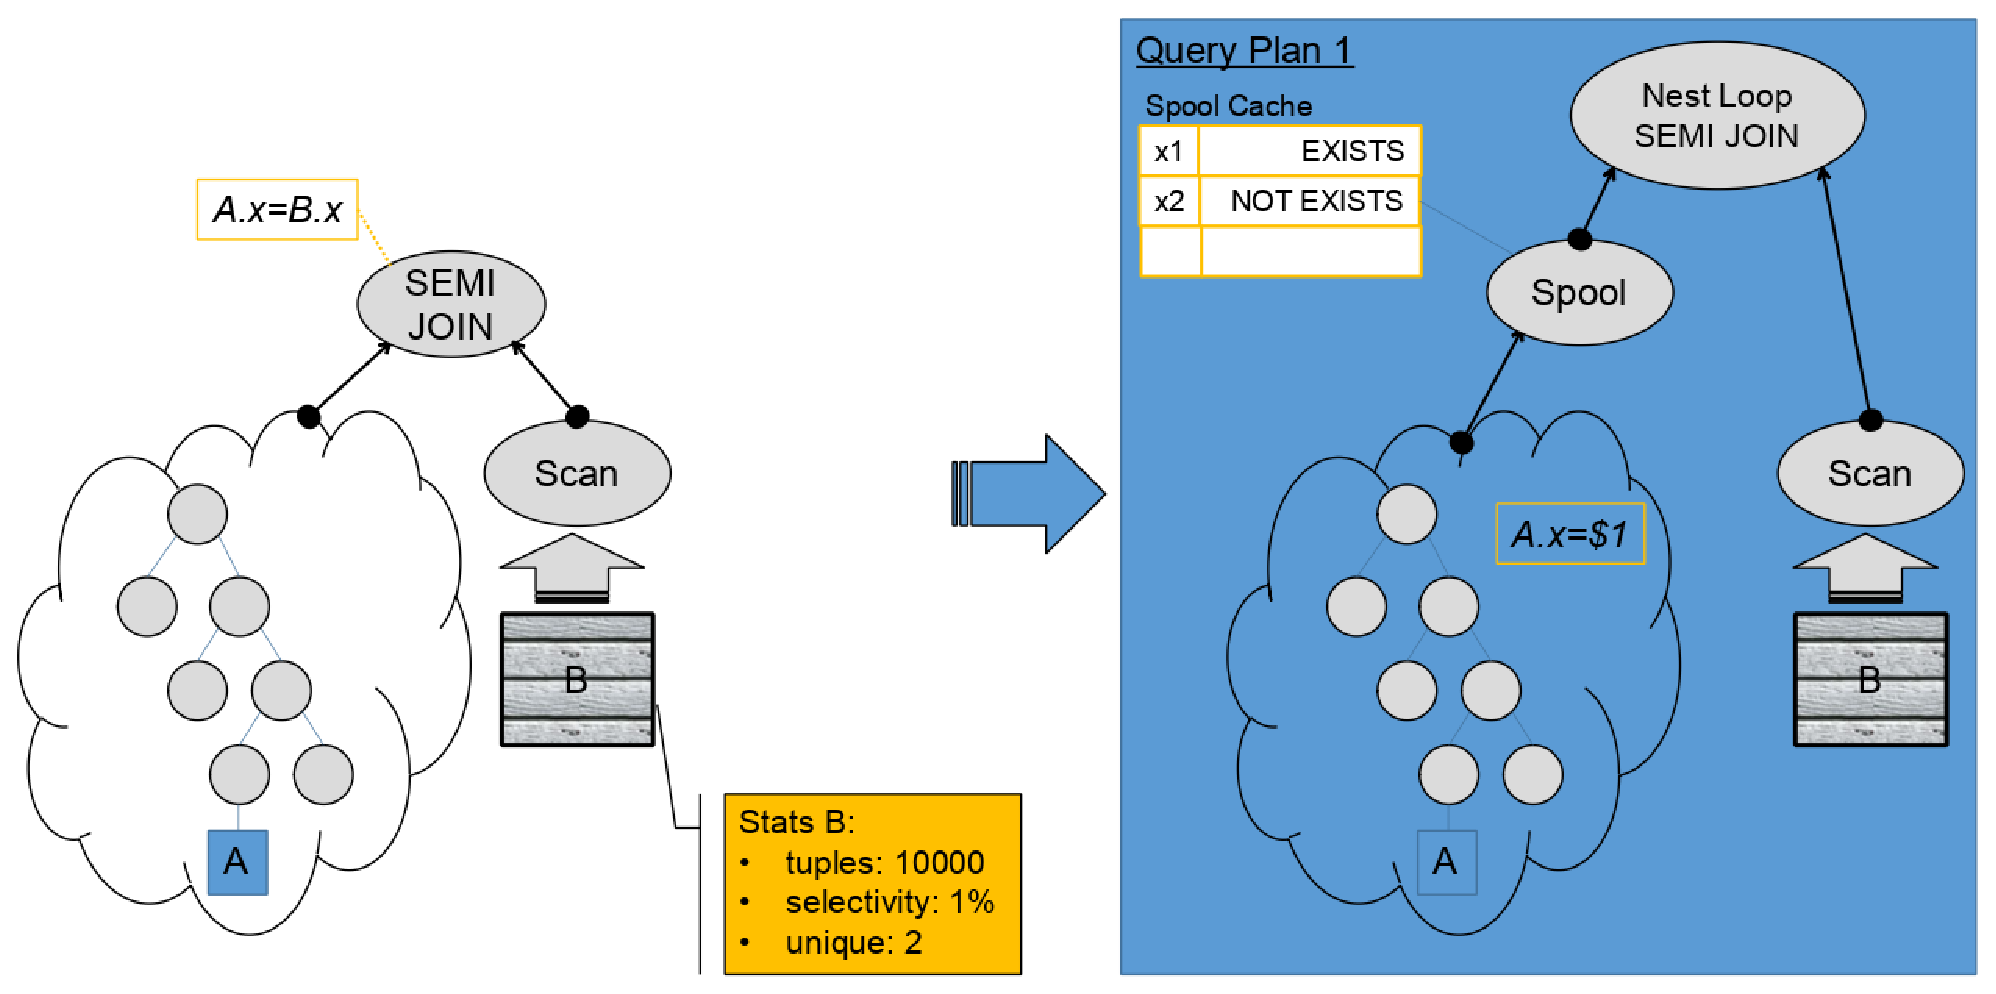
\includegraphics[scale=0.35]{pics/spool}
\hspace*{\fill}
%\end{center}
\end{frame}

\begin{frame}\frametitle{Parameters cache: example}
%\begin{center}
\hspace*{\fill}
	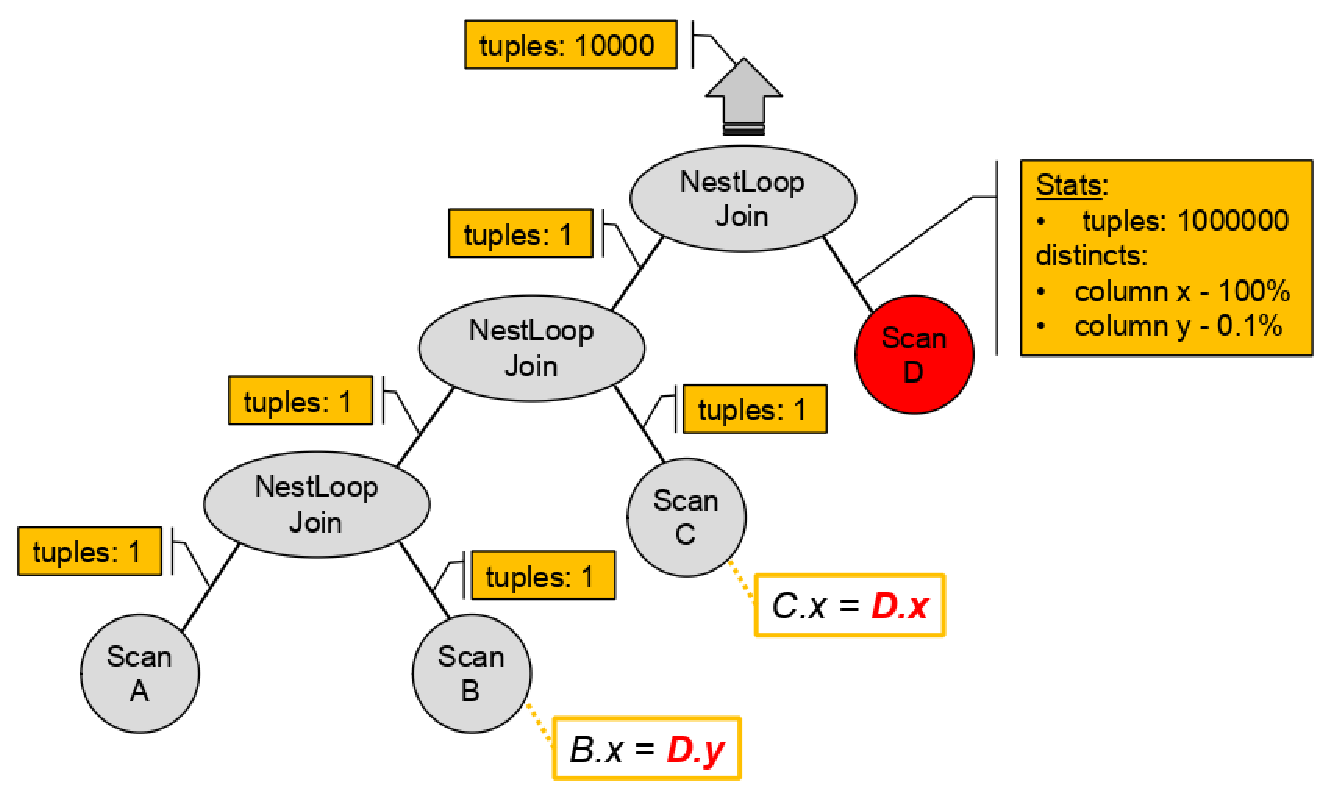
\includegraphics[scale=0.5]{pics/spool_example_1}
\hspace*{\fill}
%\end{center}
\end{frame}

\begin{frame}\frametitle{Parameters cache: example}
%\begin{center}
\hspace*{\fill}
	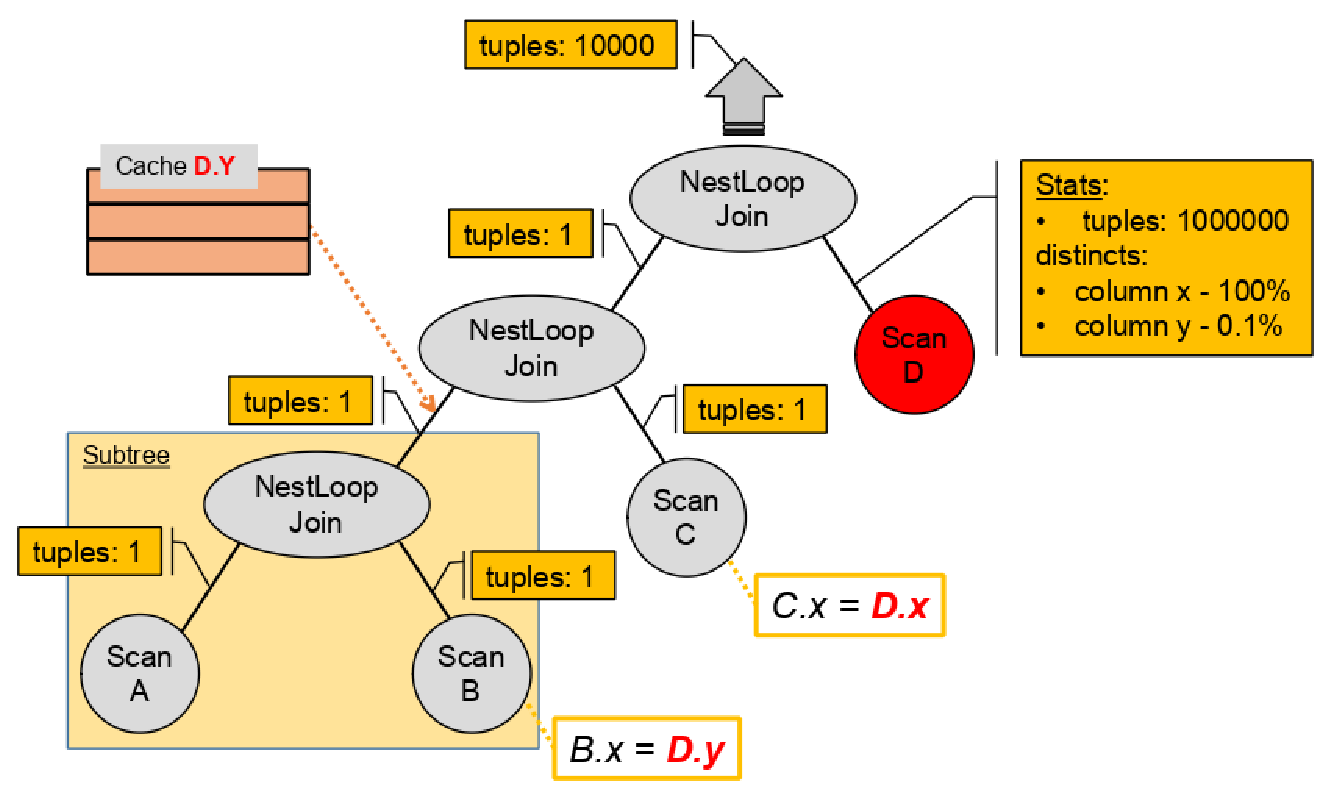
\includegraphics[scale=0.5]{pics/spool_example_2}
\hspace*{\fill}
%\end{center}
\end{frame}

\begin{frame}\frametitle{Memoization: Top-bottom planning pass needed?}
\begin{quote}
Postgres optimisation passes from base relations to the top GROUP/ORDER-BY operation. We probably need a second, top-bottom optimisation pass to find out points of frequent rescanning and insert caching (Material, Memoize) nodes. \\
Such an approach could also let us find new paths for queries with limits.
\end{quote}
\end{frame}

% %%%%%%%%%%%%%%%%%%%%%%%%%%%%%%%%%%%%%%%%%%%%%%%%%%%%%%%%%%%%%%%%%%%%%%%%

\begin{frame}
\vspace*{\fill}
\begin{center}
Subqueries \& CTE
\end{center}
\vspace*{\fill}
\end{frame}

\begin{frame}\frametitle{Subqueries \& CTE}
\begin{itemize}
  \item Subquery -> JOIN transformation
  \item Precalculated Subquery and CTE result
  \item Use subquery stat (sort order, rows number, uniqueness) at the top-query planning
  \item Choose the best-fitting subquery plan
\end{itemize}
\end{frame}

% Difference between Subquery and Subplan? We have SubqueryScan as a data source and SubPlan if it is just a parameter in an expression.

\begin{frame}[fragile]\frametitle{Unnesting Correlated Subqueries (CSQ)}
\begin{lstlisting}
SELECT * FROM t1 WHERE y IN (
  SELECT y FROM t2 WHERE t1.x=t2.x);
\end{lstlisting}

\begin{block}{BEFORE Unnesting}
\begin{lstlisting}[basicstyle=\footnotesize]
 Seq Scan on t1
   Filter: (SubPlan 1)
   SubPlan 1
     ->  Seq Scan on t2
           Filter: (t1.x = x)
\end{lstlisting}\end{block}

\begin{block}{AFTER Unnesting}
\begin{lstlisting}[basicstyle=\footnotesize]
 Nested Loop Semi Join
   Join Filter: ((t1.x = t2.x) AND (t1.y = t2.y))
   ->  Seq Scan on t1
   ->  Seq Scan on t2
\end{lstlisting}\end{block}
\end{frame}

\begin{frame}[fragile]\frametitle{CSQ - prospectives}
Postgres can transform:
\begin{lstlisting}
SELECT * FROM t1 WHERE y IN (
  SELECT y FROM t2 WHERE t1.x=t2.x);
\end{lstlisting}
The long list of possible transformations:
\begin{itemize}
  \item Subquery in select list
  \item In disjunctive filter
  \item With GROUP-BY and inequality
  \item Must return single row (equality operator)
  \item Subquery references outer side (multilevel case)
\end{itemize}
\end{frame}

\begin{frame}[fragile]\frametitle{CSQ - Just an example}
\begin{lstlisting}
CREATE UNIQUE INDEX ON t2(x);

SELECT * FROM t1 WHERE y = (
  SELECT y FROM t2 WHERE t1.x=t2.x);
\end{lstlisting}
\begin{block}{Proved single row return}
\begin{lstlisting}[basicstyle=\footnotesize]
 Seq Scan on t1
   Filter: (y = (SubPlan 1))
   SubPlan 1
     ->  Index Scan using t2_x_idx on t2
           Index Cond: (x = t1.x)
\end{lstlisting}\end{block}
\end{frame}

\begin{frame}[fragile]\frametitle{New CTE features}
Before 2024, the general idea was to isolate the planning of the query and its subplans to simplify the process. In 2024, there is a big leap ahead: propagation of sorting. \\ Example: \\
\begin{block}{EXPLAIN (COSTS OFF)}
\begin{lstlisting}
WITH x AS MATERIALIZED (
  SELECT unique1 FROM tenk1 b
  ORDER BY unique1
) SELECT count(*) FROM tenk1 a
WHERE unique1 IN (SELECT * FROM x);
\end{lstlisting}
\end{block}
\end{frame}

\begin{frame}[fragile]\frametitle{Sort info propagation - example}
\textbf{Before:}
\begin{lstlisting}
 Aggregate
   CTE x
     ->  Index Only Scan using tenk1_unique1 on tenk1 b
   ->  Nested Loop
         ->  HashAggregate
               Group Key: x.unique1
               ->  CTE Scan on x
         ->  Index Only Scan using tenk1_unique1 on tenk1 a
               Index Cond: (unique1 = x.unique1)
\end{lstlisting}
\textbf{After:}
\begin{lstlisting}
 Aggregate
   CTE x
     ->  Index Only Scan using tenk1_unique1 on tenk1 b
   ->  Merge Semi Join
         Merge Cond: (a.unique1 = x.unique1)
         ->  Index Only Scan using tenk1_unique1 on tenk1 a
         ->  CTE Scan on x
\end{lstlisting}
\end{frame}

\begin{frame}\frametitle{CTE - what's more?}
Break membrane between query and subquery planning (maybe on demand):
\begin{itemize}
  \item Expose alternative paths to the upper query
  \item Push parameters into a subquery
  \item Replan subquery if the upper query has additional info
\end{itemize}
\hspace*{\fill}
	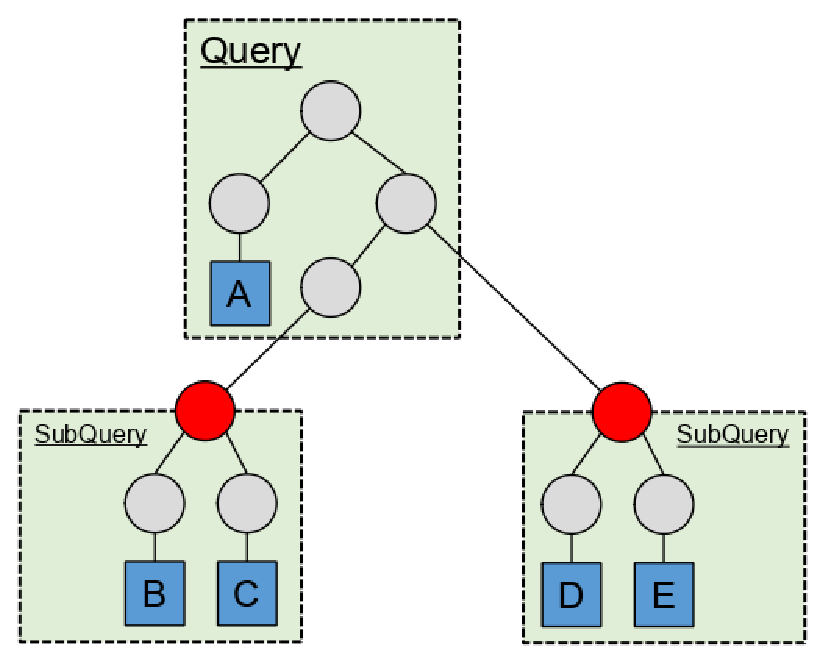
\includegraphics[scale=0.2]{pics/subplan_membrane}
\end{frame}

% %%%%%%%%%%%%%%%%%%%%%%%%%%%%%%%%%%%%%%%%%%%%%%%%%%%%%%%%%%%%%%%%%%%%%%%%

\begin{frame}
\vspace*{\fill}
\begin{center}
Indexes ?
\end{center}
\vspace*{\fill}
\end{frame}

\begin{frame}[fragile]\frametitle{Indexes as an optimisation tool}
2010 - inequality estimations with indexes:
\begin{lstlisting}
SELECT * FROM table WHERE x < 5;
\end{lstlisting}
\begin{center}
  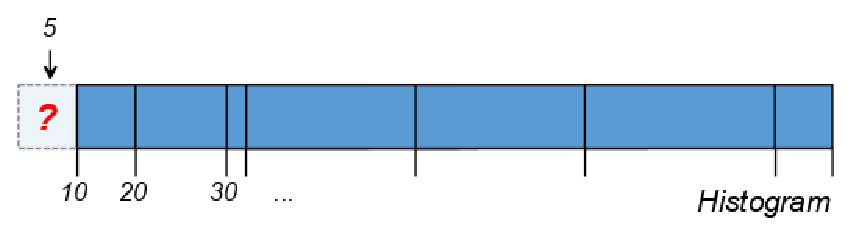
\includegraphics[scale=0.5]{pics/histogram}
\end{center}
Optimiser fetches index tuples to estimate cardinality in cases:
\begin{itemize}
  \item Histogram too simple
  \item The value hits the first (last) histogram bin
  \item The value out of the histogram
\end{itemize}
\end{frame}

\begin{frame}[fragile]\frametitle{What's more with indexes}
Index estimation is a promising way to tackle optimistic '1-tuple' estimations.
\begin{itemize}
  \item Direct index fetch is too heavy
  \item Change Access Method interface to allow index estimations based on the number of pages/average width data.
  \item Implement Index Estimation for equalities
  \item Multi-clause filters estimations covered by an index
\end{itemize}
\end{frame}


% %%%%%%%%%%%%%%%%%%%%%%%%%%%%%%%%%%%%%%%%%%%%%%%%%%%%%%%%%%%%%%%%%%%%%%%%

\begin{frame}
\vspace*{\fill}
\begin{center}
Aggregates \& Window Functions
\end{center}
\vspace*{\fill}
\end{frame}

\begin{frame}[fragile]\frametitle{Aggregates \& Window Functions}
\begin{itemize}
  \item Hashed Aggregates
  \item Combine aggregate's sort orders
  \item Prosupport machinery
\end{itemize}
\end{frame}

\begin{frame}[fragile]\frametitle{Hashed Aggregates}
  \centerline{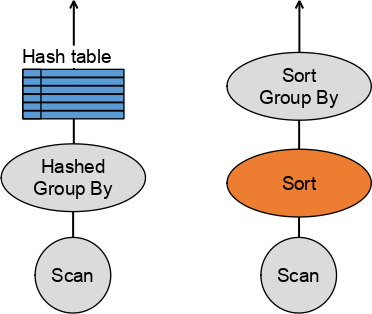
\includegraphics[scale=0.7]{pics/hashed_groupby.png}}
\end{frame}

\begin{frame}[fragile]\frametitle{Combine sortings}
\begin{lstlisting}[basicstyle=\tiny]
SELECT sum(unique1 ORDER BY ten), sum(unique1 ORDER BY ten,two)
FROM tenk1 GROUP BY ten;
\end{lstlisting}
Execution plans:
  \centerline{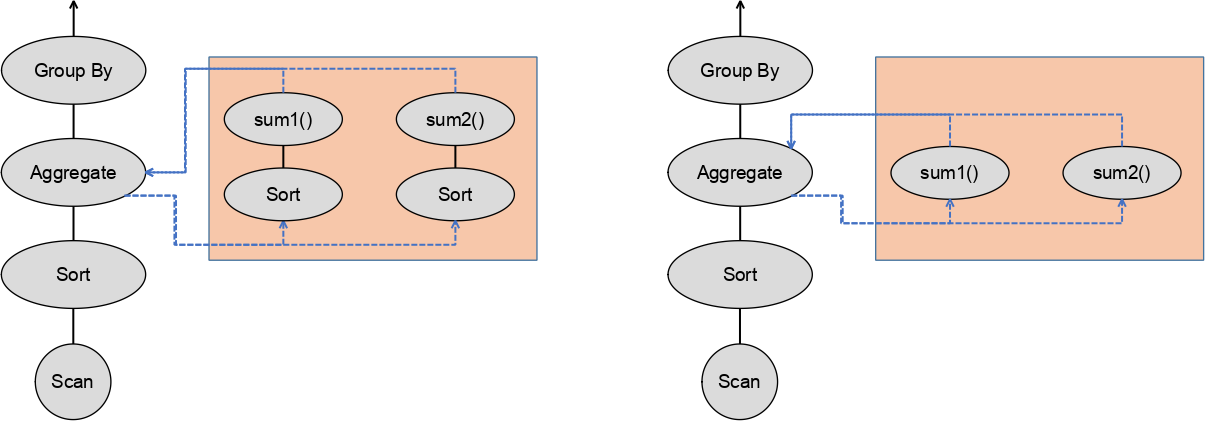
\includegraphics[scale=0.35]{pics/aggsort.png}}
\end{frame}

\begin{frame}[fragile]\frametitle{Combine sortings}
\begin{lstlisting}[basicstyle=\tiny]
EXPLAIN (ANALYZE, TIMING OFF, COSTS ON)
SELECT sum(unique1 ORDER BY ten), sum(unique1 ORDER BY ten,two)
FROM tenk1 GROUP BY ten;

-- PG13:

GroupAggregate  (cost=1108.97..1209.02) (actual rows=10 loops=1)
  Output: sum(unique1 ORDER BY ten), sum(unique1 ORDER BY ten, two), ten
  Group Key: tenk1.ten
  ->  Sort  (cost=1108.97..1133.95) (actual rows=10000 loops=1)
        Output: ten, unique1, two
        Sort Key: tenk1.ten
        ->  Seq Scan on public.tenk1  (cost=0.00..444.95)
              Output: ten, unique1, two
Execution Time: 116.375 ms

-- PG17:

GroupAggregate  (cost=1109.39..1209.49) (actual rows=10 loops=1)
  Output: sum(unique1 ORDER BY ten), sum(unique1 ORDER BY ten, two), ten
  Group Key: tenk1.ten
  ->  Sort  (cost=1109.39..1134.39) (actual rows=10000 loops=1)
        Output: ten, unique1, two
        Sort Key: tenk1.ten, tenk1.two
        ->  Seq Scan on public.tenk1  (cost=0.00..445.00)
              Output: ten, unique1, two
Execution Time: 12.650 ms
\end{lstlisting}
\end{frame}
% What to improve in that area? This part of the code isn't popular and looks
% like a big mess for now. - Maybe we need some explanation and a cost model here.

\begin{frame}[fragile]\frametitle{Prosupport machinery}
\begin{itemize}
  \item A function has been a black box for the planner: rows? cost? selectivity? ...
  \item Postgres community respond to the challenge - prosupport
  \item Prosupport - routine which can be attached to any stored procedure
  \item At the planning stage, Prosupport can provide cost, rows, selectivity recommendations
  \item full function replacement, index condition
  \item Window function optimisations
\end{itemize}
\end{frame}

\begin{frame}[fragile]\frametitle{Prosupport machinery - an example}
\begin{lstlisting}[basicstyle=\tiny]
PREPARE stmt(int) AS SELECT x FROM test WHERE int4mul(x, $1) < 100;

EXECUTE stmt(0);
                                   QUERY PLAN                                    
----------------------------------------------------------------------------------
 Seq Scan on test  (cost=0.00..20.00 rows=333 width=4) (actual rows=1000 loops=1)
   Filter: (int4mul(x, 0) < 100)

EXECUTE stmt(1);
                                   QUERY PLAN                                   
--------------------------------------------------------------------------------
 Seq Scan on test  (cost=0.00..20.00 rows=333 width=4) (actual rows=99 loops=1)
   Filter: (int4mul(x, 1) < 100)

EXECUTE stmt(2);
                                   QUERY PLAN                                   
--------------------------------------------------------------------------------
 Seq Scan on test  (cost=0.00..20.00 rows=333 width=4) (actual rows=49 loops=1)
   Filter: (int4mul(x, 2) < 100)
\end{lstlisting}
\end{frame}

\begin{frame}[fragile]\frametitle{Prosupport machinery - use help routine}
\begin{lstlisting}[basicstyle=\tiny]
UPDATE pg_proc SET prosupport = 'int4mul_support' WHERE proname = 'int4mul';
PREPARE stmt(int) AS SELECT x FROM test WHERE int4mul(x, $1) < 100;

EXECUTE stmt(0);
                                    QUERY PLAN                                     
-----------------------------------------------------------------------------------
 Seq Scan on test  (cost=0.00..15.00 rows=1000 width=4) (actual rows=1000 loops=1)

EXECUTE stmt(1);
                                  QUERY PLAN                                   
-------------------------------------------------------------------------------
 Seq Scan on test  (cost=0.00..17.50 rows=99 width=4) (actual rows=99 loops=1)
   Filter: (x < 100)

EXECUTE stmt(2);
                                   QUERY PLAN                                   
--------------------------------------------------------------------------------
 Seq Scan on test  (cost=0.00..20.00 rows=333 width=4) (actual rows=49 loops=1)
   Filter: (int4mul(x, 2) < 100)
\end{lstlisting}
\end{frame}

\begin{frame}[fragile]\frametitle{Prosupport - usage}
\centerline{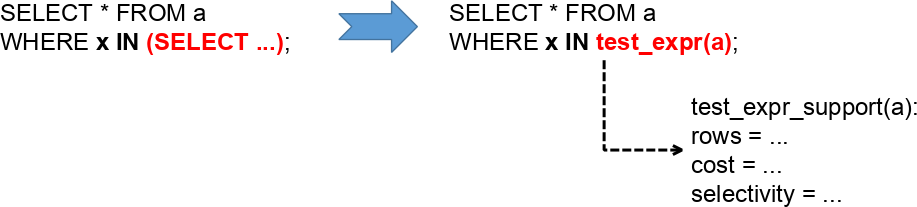
\includegraphics[scale=0.45]{pics/prosupport.png}}
\end{frame}

\begin{frame}[fragile]\frametitle{Prosupport - what's more?}
\begin{itemize}
  \item Prosupport for aggregates
  \item Same technique for Query tree nodes?
  \item Sublink, Coalesce, BoolExpr - can we register prosupport routines to transform them on-demand?
\end{itemize}
\end{frame}

% %%%%%%%%%%%%%%%%%%%%%%%%%%%%%%%%%%%%%%%%%%%%%%%%%%%%%%%%%%%%%%%%%%%%%%%%

\begin{frame}
\vspace*{\fill}
\begin{center}
Query structure
\end{center}
\vspace*{\fill}
\end{frame}

\begin{frame}[fragile]\frametitle{Manage complex Query}
\begin{itemize}
  \item Multiple joins
  \item Minimize of sort operations
  \item Left Joins and inner-generated NULLS
  \item Multicolumn statistics
\end{itemize}
\end{frame}

\begin{frame}[fragile]\frametitle{Incremental Sort}
\begin{lstlisting}
CREATE INDEX idx1 ON test (x);
CREATE INDEX idx2 ON test (x,y);
SELECT x,y,z FROM test ORDER BY x,y,z;
\end{lstlisting}
  \centerline{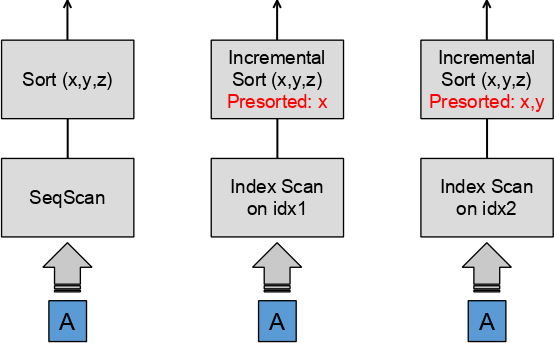
\includegraphics[scale=0.6]{pics/incremental_sort.png}}
\end{frame}

\begin{frame}[fragile]\frametitle{Minimize of sort operations}
\begin{lstlisting}
SELECT x,y,z FROM test ORDER BY x,y,z;
\end{lstlisting}
\begin{block}{Full sort plan}
\begin{lstlisting}[basicstyle=\tiny]
 Sort  (cost=9845.82..10095.82 rows=100000 width=12)
   Sort Key: x, y, z
   ->  Seq Scan on test  (cost=0.00..1541.00 rows=100000 width=12)
\end{lstlisting}
\end{block}
\begin{block}{Exploit presorted column x}
\begin{lstlisting}[basicstyle=\tiny]
 Incremental Sort  (cost=7.62..8599.52 rows=100000 width=12)
   Sort Key: x, y, z
   Presorted Key: x
   ->  Index Scan using test_x_idx on test  (cost=0.29..4007.59 rows=100000 width=12)
\end{lstlisting}
\end{block}
\begin{block}{Exploit presorted columns x and y}
\begin{lstlisting}[basicstyle=\tiny]
 Incremental Sort  (cost=0.86..7118.86 rows=100000 width=12)
   Sort Key: x, y, z
   Presorted Key: x, y
   ->  Index Scan using test_x_y_idx on test  (cost=0.29..4007.90 rows=100000 width=12)
\end{lstlisting}
\end{block}
\end{frame}

\begin{frame}[fragile]\frametitle{Sort - what's more?}
\begin{lstlisting}[basicstyle=\scriptsize]
EXPLAIN SELECT x,y,z FROM test ORDER BY x,y;

                                   QUERY PLAN                                   
--------------------------------------------------------------------------------
 Incremental Sort  (cost=42.85..9765.17 rows=100000 width=12)
   Sort Key: x, y
   Presorted Key: x
   ->  Index Scan using idx1 on test  (cost=0.29..4028.28 rows=100000 width=12)

EXPLAIN SELECT x,y,z FROM test ORDER BY x,y,z;

                                   QUERY PLAN                                   
--------------------------------------------------------------------------------
 Incremental Sort  (cost=42.85..9765.17 rows=100000 width=12)
   Sort Key: x, y, z
   Presorted Key: x
   ->  Index Scan using idx1 on test  (cost=0.29..4028.28 rows=100000 width=12)
\end{lstlisting}
\end{frame}
% We have not touched it for many years because we are dealing with short queries.
% Here, the general idea is that the number of sort keys and order of sorting saves comparison operator calls, and it may be crucial in analytic queries when we extract data in the very early stages of query execution and many times manipulate it afterwards.

% Sortings initially went from the PGPRO-8491 - we can have lots of sortings because of pulling up subqueries.

\begin{frame}[fragile]\frametitle{NULLs Counting Problem}
  \centerline{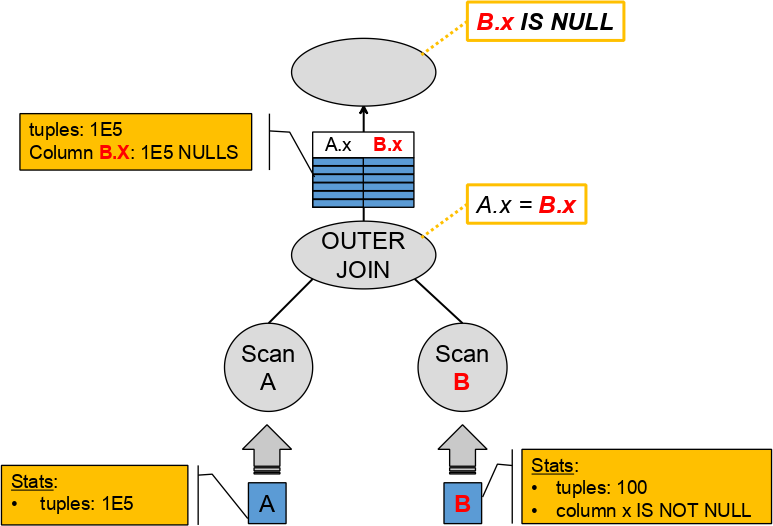
\includegraphics[scale=0.4]{pics/nulls_counting.png}}
\end{frame}

\begin{frame}[fragile]\frametitle{NULLs Counting Problem - levels}
  \centerline{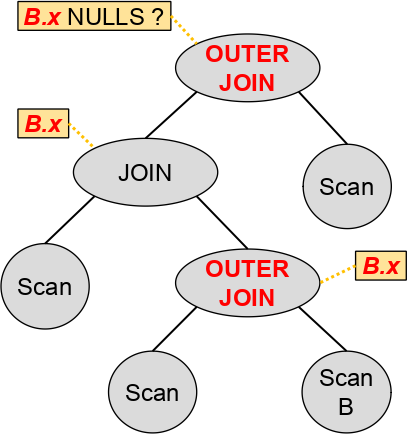
\includegraphics[scale=0.55]{pics/nulls_levels.png}}
\end{frame}

\begin{frame}[fragile]\frametitle{NULLs Counting Problem - join types}
\begin{columns}\begin{column}{0.5\textwidth}
\begin{lstlisting}
EXPLAIN (COSTS OFF)
SELECT oid, relname
FROM pg_class c1
  LEFT JOIN pg_class c2
  ON c1.relname = c2.relname;

 Hash Left Join
   Hash Cond: (c1.relname = c2.relname)
   ->  Seq Scan on pg_class c1
   ->  Hash
         ->  Seq Scan on pg_class c2
\end{lstlisting}
\end{column}\begin{column}{0.5\textwidth}
\begin{lstlisting}
EXPLAIN (COSTS OFF)
SELECT c1.oid, c1.relname
FROM pg_class c1
  LEFT JOIN pg_class c2 ON true
  WHERE c1.relname = c2.relname;

 Hash Join
   Hash Cond: (c1.relname = c2.relname)
   ->  Seq Scan on pg_class c1
   ->  Hash
         ->  Seq Scan on pg_class c2
\end{lstlisting}
\end{column}\end{columns}
\end{frame}
% %%%%%%%%%%%%%%%%%%%%%%%%%%%%%%%%%%%%%%%%%%%%%%%%%%%%%%%%%%%%%%%%%%%%%%%%%%%%%%
%
% Extended Statistics short introduction
%
% %%%%%%%%%%%%%%%%%%%%%%%%%%%%%%%%%%%%%%%%%%%%%%%%%%%%%%%%%%%%%%%%%%%%%%%%%%%%%%

\begin{frame}[fragile]\frametitle{Extended Statistics}
\begin{lstlisting}
SELECT * FROM table WHERE id IN (1,2,3,4,5) AND enabled = true AND
  status = 'ready';

Selectivity 'id IN (1,2,3,4,5)' -> 0.00001
Selectivity 'enabled = true' -> 0.5
Selectivity 'status = ready' -> 0.1
Selectivity of the whole clause - ?
\end{lstlisting}
\end{frame}

\begin{frame}[fragile]\frametitle{Extended Statistics}
\vskip0pt plus 1filll
CREATE STATISTICS ON id,enabled,status FROM tablename;
\vspace{10pt}
\begin{itemize}
  \item \textbf{MCV} - \textbf{M}ost \textbf{C}ommon \textbf{V}alues on composite value  of (x1,x2,x3).
  \item \textbf{ndistinct} - number of distinct values on all combinations of columns: (x1,x2),(x1,x3),(x1,x2,x3)...
  \item \textbf{dependencies} - functional dependencies between combinations of columns: x1->x2, (x1,x2)->x3,...
\end{itemize}
\vskip0pt plus 1filll
\begin{columns}\begin{column}{0.03\textwidth}

\includegraphics[scale=0.1]{pics/vondra_extstat}
\end{column}\begin{column}{0.8\textwidth}
\textit{Vondra. T. CREATE STATISTICS improvements,\\ PGConf.DE 2022}
\end{column}\end{columns}
\end{frame}
%I want to explain the extended statistic a bit to ensure we are on the same page. The best description of that feature can be found in Tomas Vondra's recent presentation (see link below). He is the leading developer of this feature. You can find it by following the link in the QR code.
%This type of statistic is designed to provide information about the joint distribution of a set of columns or expressions. At the top of the slide, you can see an example of its definition. Currently, extended statistics can be built upon one table involving some columns or expressions.
%These statistics are still not extensible and include three types of data: most common values, number of distinct values and dependency factor.
%The MCV is a collection of the most frequent values. The number of distinct values is calculated for all possible combinations of the defining columns and dependency shows us the dependency factor between any possible combination of columns in the set of columns. 

\begin{frame}[fragile]\frametitle{Laboriousness of Extended Statistics}
\begin{itemize}
  \item \textbf{MCV} - two arrays: values[] and frequences[].
  \item \textbf{ndistinct} - 1 integer for each of $2^n - (n+1)$ combinations
  \item \textbf{dependencies} - 1 float value for each of combinations
\end{itemize}
\vspace{20pt}
\begin{center}
\begin{tabular}{|l|c|c|c|c|c|}
\hline
columns: & 2 & 3 & 4 & ... & 8 \\
\hline
distinct combinations: & 1 & 4 & 11 & ... & 247 \\
\hline
dependency combinations: & 2 & 9 & 28 & ... & 1016 \\
\hline
\end{tabular}
\end{center}
\end{frame}
% Let's see the complexity of maintaining such statistics in the actual state.
%MCV is an array of data values and another one for their frequency. Here, frequencies are fixed-length real values. But data in the column, especially composite one can be lengthy and add overhead on detoasting.
%The ndistinct is just one number for whole column and only adds a little overhead to reading and writing from the catalog. However, the number of combinations is growing fast with the number of columns involved. Here, you can see the exact numbers of such combinations. With 8 columns, we must calculate it for 247 combinations during analysis.
%It's the same with dependencies. Even worse, for 8 columns, we must generate around 1000 combinations. It may be expensive.
%Taking all the above facts into account, I think we should somehow separate the ANALYZE of plain and extended statistics. Or, at least, add a parameter to the analyse command.
% KEY IDEA: separation from plain statistics and be careful about that.

% %%%%%%%%%%%%%%%%%%%%%%%%%%%%%%%%%%%%%%%%%%%%%%%%%%%%%
%
% Rationale for the usage of indexes. An example.
%
% %%%%%%%%%%%%%%%%%%%%%%%%%%%%%%%%%%%%%%%%%%%%%%%%%%%%%
\begin{frame}[fragile]\frametitle{Index to define statistics}
\begin{lstlisting}[basicstyle=\footnotesize]
Table "Parcels":
Indexes:
    "parcel_pkey" PRIMARY KEY, btree (id)
    "parcel_parcel_id" btree (parcel_id)
    "parcel_id_prik" btree (parcel_id, prik)
    "parcel_id_sn_pol" btree (parcel_id, sn_pol)
    "parcel_par_begin" btree (parcel_id, prik_begin_period)
    "parcel_par_patient" btree (parcel_id, patient_id)
    "parcel_par_recid" btree (parcel_id, recid)
    "parcel_per_prik" btree (period, prik)
\end{lstlisting}
\end{frame}

\begin{frame}[fragile]\frametitle{Extended statistics - what's more?}
\begin{itemize}
  \item Extended statistics for JOINs
  \item Reduction of combinations inside Distinct and Dependencies based on index definition
  \item New methods - multidimensional histogram
\end{itemize}
\end{frame}
% %%%%%%%%%%%%%%%%%%%%%%%%%%%%%%%%%%%%%%%%%%%%%%%%%%%%%%%%%%%%%%%%%%%%%%%%

\begin{frame}
\vspace*{\fill}
\begin{center}
Miscellaneous optimisations
\end{center}
\vspace*{\fill}
\end{frame}

\begin{frame}[fragile]\frametitle{Miscellaneous optimisations - examples}
\begin{itemize}
  \item VALUES -> ANY transformation
  \item OR list -> ANY transformation
  \item GROUP-BY makes column 'unique'
  \item Static functions evaluation
  \item ...
\end{itemize}
\end{frame}

\begin{frame}[fragile]\frametitle{Miscellaneous optimisations - VALUES -> ANY}
\begin{columns}[T]\begin{column}{0.5\textwidth}
\begin{lstlisting}
SELECT * FROM a
WHERE a.x IN (VALUES (1), (2), (3));
\end{lstlisting}
\end{column}\begin{column}{0.5\textwidth}
\begin{lstlisting}
SELECT * FROM a
WHERE a.x = ANY ('{1,2,3}');
\end{lstlisting}
\end{column}\end{columns}
\begin{columns}[T]\begin{column}{0.5\textwidth}
\begin{block}{BEFORE transformation}
\begin{lstlisting}
 Hash Semi Join
   Hash Cond:
     (a.x = "*VALUES*".column1)
   ->  Seq Scan on a
   ->  Hash
         ->  Values Scan on
                       "*VALUES*"
\end{lstlisting}
\end{block}
\vspace*{\fill}
\end{column}\begin{column}{0.5\textwidth}
\begin{block}{AFTER transformation}
\begin{lstlisting}
 Seq Scan on a
   Filter:
     (x = ANY ('{1,2,3}'::integer[]))
\end{lstlisting}
\end{block}
\vspace*{\fill}
\end{column}\end{columns}
\end{frame}

\begin{frame}[fragile]\frametitle{Miscellaneous optimisations - GROUP-BY}
\begin{columns}[T]\begin{column}{0.6\textwidth}
  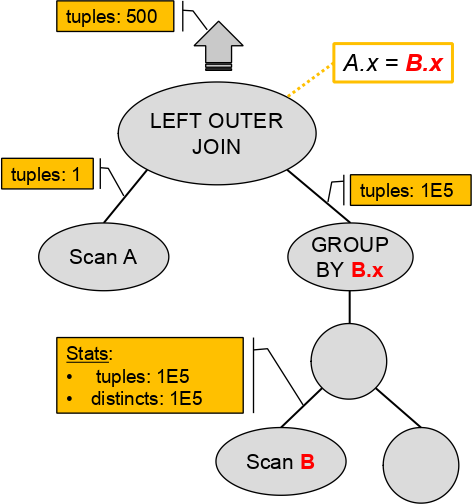
\includegraphics[scale=0.5]{pics/group-by-unique.png}
\end{column}\begin{column}{0.4\textwidth}
GROUP-BY makes grouped column 'almost' unique. We can use at in cardinality estimations.
\end{column}\end{columns}
% Knowing nothing about distribution of grouped data it uses ndistinct = 200
\end{frame}

\begin{frame}[fragile]\frametitle{Miscellaneous optimisations - pro \& cons}
\begin{itemize}
  \item It may be dozens of such optimisations
  \item Have quite a narrow application
  \item May add a lot of overhead in general case
  \item May hide better query plans
  \item Complicates the core code
\end{itemize}
\end{frame}

\begin{frame}[fragile]\frametitle{Miscellaneous optimisations - resume}
Let extensions do it!
\begin{itemize}
  \item Query transformation hooks
  \item Selectivity estimation/statistics hooks
  \item Optimisation stages hooks
  \item the add\_path hooks
  \item EXPLAIN node hook
  \item Extensible parts in the planner structures: PlannerInfo, Query and PlanStatement nodes
\end{itemize}
\end{frame}

% %%%%%%%%%%%%%%%%%%%%%%%%%%%%%%%%%%%%%%%%%%%%%%%%%%%%%%%%%%%%%%%%%%%%%%%%

\begin{frame}
\vspace*{\fill}
\begin{center}
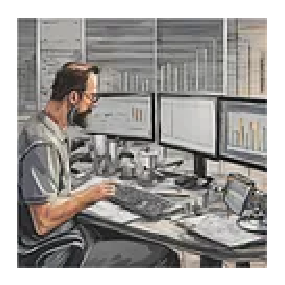
\includegraphics[scale=0.5]{pics/project_logo}\\
\huge{Questions ?}
\end{center}
\vspace*{\fill}
\begin{center}

\includegraphics[scale=0.1]{pics/url-supplement.png}
\end{center}
\end{frame}

%\begin{frame}\frametitle{Enforce partition pruning?}
%\end{frame}

\end{document}
